%\documentclass[twoside,twocolumn,spanish]{article}
\documentclass{article}
\usepackage[T1]{fontenc}
\usepackage[utf8]{inputenc}
\usepackage{graphicx}
\usepackage[spanish]{babel}
\usepackage{amssymb,amsmath,geometry,multicol,spalign,hyperref}
\setlength\columnsep{20pt}
\usepackage[usenames,dvipsnames]{xcolor}
\usepackage{tikz,mathtools}
\usepackage{circuitikz}
\usepackage{pgfplots}
\pgfplotsset{width=5cm,compat=1.12}
\usepgfplotslibrary{fillbetween}

\title{Difrentes metodos de medida de resistencias y curva carcterística de una bombilla}
\author{Andoni Latorre Galarraga \\ \href{mailto:alatorre73@alumno.uned.es}{alatorre73@alumno.uned.es}}
\date{}
\begin{document}

\maketitle
\begin{abstract}
Se exploran diferente maneras de medir resistencia de manera indirecta,: montaje corto y montaje largo. También se obtiene la curva característica de una bombilla. El experimento se ha relaiza siguiendo las indicaciones de \cite{web}.
\end{abstract}

\begin{multicols}{2}

\section*{Fundamento Teórico}
\subsection*{Ley de Ohm}
\begin{center}
\begin{circuitikz}
\draw (0,0) to[ american resistor , l=$R$] (4,0) to[ short , l=$I$] (4,-1) to[ battery1 , l=$\varepsilon$ ] (0,-1) -- (0,0); 
\end{circuitikz}
\end{center}
La ley de Ohm dice que la diferencia de potencial entre ambos bornes de un conductor, $\varepsilon$, es igual al producto de la resistencia de dicho conductor, $R$, y la intensidad de la corriente, $I$.
$$
\varepsilon = I R
$$
\subsection*{Amperiemetros y Voltímetros}
\subsubsection*{Amperimetros}
Los amperimetros se conectan en serie con la corriente que se quiere medir. Los amperimetros suelen tener una resistencia interna del orden de $1\Omega$ y normalmente no afectan al circuito ya que la corriente pasa por ellos sin problema. Sin embargo cuando se esta utilizando un circuito con resistencias del orden de la resistencia interna del amperimetro, es decir, resitencias muy pequeñas, este puede influir sgnificativamente en las mediciones. Ya que la corriente no pasará por el amperimetro.
\subsubsection*{Voltímetros}
Los voltímetros se conectan en paralelo a la corriente que se quiere medir. Los voltímetros suelen tener una resistencia interna del orden de $1M\Omega$ y normalmente no afectan al circuito ya que la corriente no pasa por ellos. Sin embargo cuando se esta utilizando un circuito con resistencias del orden de la resistencia interna del voltímetro, es decir, resitencias muy grandes, este puede influir sgnificativamente en las mediciones. Ya que la corriente pasara por el voltímetro.
\subsection*{Medida indirecta de una resistencia}
Una resistencia se puede medir indirectamente, midiendo el voltaje y la intensidad para luego usar la ley de Ohm. Esto se puede hacer de dos maneras:
Ambos montajes tienen sus fallos cuando no se consideran las resistencias internas.
\subsubsection*{Montaje corto}
\begin{center}
  \begin{circuitikz}
    \node at (3.5,0.5){Montaje corto};
    \draw (1,1) -- (4.5,1) -- (4.5,2.25) circle [radius = 10pt]node[circle,fill=white,minimum size=10pt]{V} (4.5,2.25) -- (4.5,3.5) -- (3,3.5) circle [radius = 10pt]node[circle,fill=white,minimum size=10pt]{A} (3,3.5) -- (1,3.5);
    \draw (1,1) to[battery1, l=$\varepsilon$] (1,3.5);
    \draw (4.5,3.5) -- (6,3.5) to[ american resistor , l_=$R$] (6,1) -- (4.5,1);
  \end{circuitikz}
\end{center}
En el montaje corto, el amperimetro no mide la intensidad que pasa por la resistencia. Por las leyes de Kirchhoff, mide la intensidad que pasa por la resistencia más la que pasa por el voltimetro. En principio esto no debe afectar mucho a la medición, por la gran resitencia interna del voltimetro. Sin embargo está claro que a medida que la resistencia $R$ se acerca al orden de la resistencia interna del voltimetro se va a producir un error sistemático significativo. El montaje corto será más preciso para valores pequeños de $R$.
\subsubsection*{Montaje largo}
\begin{center}
  \begin{circuitikz}
    \node at (3.5,0.5){Montaje largo};
    \draw (1,1) -- (3,1) -- (3,2.25) circle [radius = 10pt]node[circle,fill=white,minimum size=10pt]{V} (3,2.25) -- (3,3.5) -- (3,3.5) -- (4.5,3.5) circle [radius = 10pt]node[circle,fill=white,minimum size=10pt]{A} (4.5,3.5) -- (6,3.5);
    \draw (1,1) to[battery1, l=$\varepsilon$] (1,3.5) -- (3,3.5);
    \draw (6,3.5) to[ american resistor , l_=$R$] (6,1) -- (3,1);
  \end{circuitikz}
\end{center}
En el montaje largo, el voltímetro no mide la diferencia de potencial entre ambos bornes de la resistencia. Mide la diferencia de potencial a ambos lados del conjunto amperimetro + resistencia. Al estar conectadas en seire las resistecias se tiene $R_{total} = R_i + R$ y $V = I(R_i + R)$. Como la resistencia interna del amperímetro, $R_i$ es muy pequeña, el efecto que tiene en la medición del voltímetro es insignificativo. Sin embargo, para valores suficientemente pequeños de $R$, el efecto de la resistencia interna va a ser significativo y va a causar un error sistemático. El montaje largo será más preciso para valores grandes de $R$.
\section*{Dispositivo Experimental, Procedimiento y Resultados}
Se han medido indirectamente resistecias etiquetadas con $50\Omega, 1K\Omega, 1M\Omega$ utilizando ambos montajes, luego se ha calculado la resistencia con la ley de Ohm.
\begin{center}
  Tabla 1: Montaje corto
  $$
  \begin{array}{|l||l|l|l|}\hline
    & V(V) & I(A) & R(\Omega) \\ \hline \hline
  50 \Omega & 4.77 & 0,0960 & 49.69 \\ \hline
  1K \Omega & 2.08 & 0.0028 & 742.85 \\ \hline
  1M \Omega & 2.09 & 0.0 & \\ \hline
  \end{array}
  $$
  Tabla 2: Montaje largo
  $$
  \begin{array}{|l||l|l|l|}\hline
    & V(V) & I(A) & R(\Omega) \\ \hline \hline
  50 \Omega & 4.97 & 0,0962 & 48.85 \\ \hline
  1K \Omega & 3.45 & 0.0048  & 718.75\\ \hline
  1M \Omega & 0.0 & 0.0  & \\ \hline
  \end{array}
  $$
\end{center}
En segundo lugar, hemos conectado dos resitencias de $47\Omega$ en serie y hemos medido la diferencia de potencial entre los bornes de la primera reistencia, $V_1$; entre los de la segunda, $V_2$ y de todo el conjunto $V_3$.
$$
V_1 = 4.99 V \quad V_2 = 4.97 V \quad V_3 = 9.91 V
$$
Finalmente hemos tomado una bombilla y hemos medido directamente su resistemcia, $2.630 \Omega$. Luego hemos medido indirectamente la resistecia. Los datos son los siguientes.
\begin{center}
  Tabla 3:
  $$
  \begin{array}{|l|l|l|} \hline
    V(mV) & I(mA) & V/I(\Omega) \\ \hline \hline
    9.5 & 0.03 & 316.67  \\ \hline
    18.8 & 0.09 & 208.89  \\ \hline
    27.4 & 0.19 & 144.21  \\ \hline
    36.1 & 0.32 & 112.81  \\ \hline
    41.1 & 0.41 & 100.24  \\ \hline
    54.4 & 0.45 & 120.89  \\ \hline
    64.1 & 0.49 & 130.82  \\ \hline
    74.8 & 0.48 & 155.83  \\ \hline
    83.9 & 0.53 & 158.3  \\ \hline
    93.6 & 0.56 & 167.14  \\ \hline
    103.6 & 0.55 & 188.36  \\ \hline
    113.8 & 0.62 & 183.55  \\ \hline
    123.6 & 0.67 & 184.48  \\ \hline
    133.4 & 0.76 & 175.53  \\ \hline
    142.9 & 0.87 & 1313.68  \\ \hline
    152.7 & 0.98 & 155.82  \\ \hline
    162.4 & 1.09 & 148.99  \\ \hline
    172.2 & 1.21 & 142.31  \\ \hline
    188.1 & 1.34 & 140.37  \\ \hline
    192.2 & 1.48 & 129.86  \\ \hline
    \end{array}
  $$
\end{center}
Mostramos en la siguiente figura la curva característica de la bombilla.
\begin{center}
  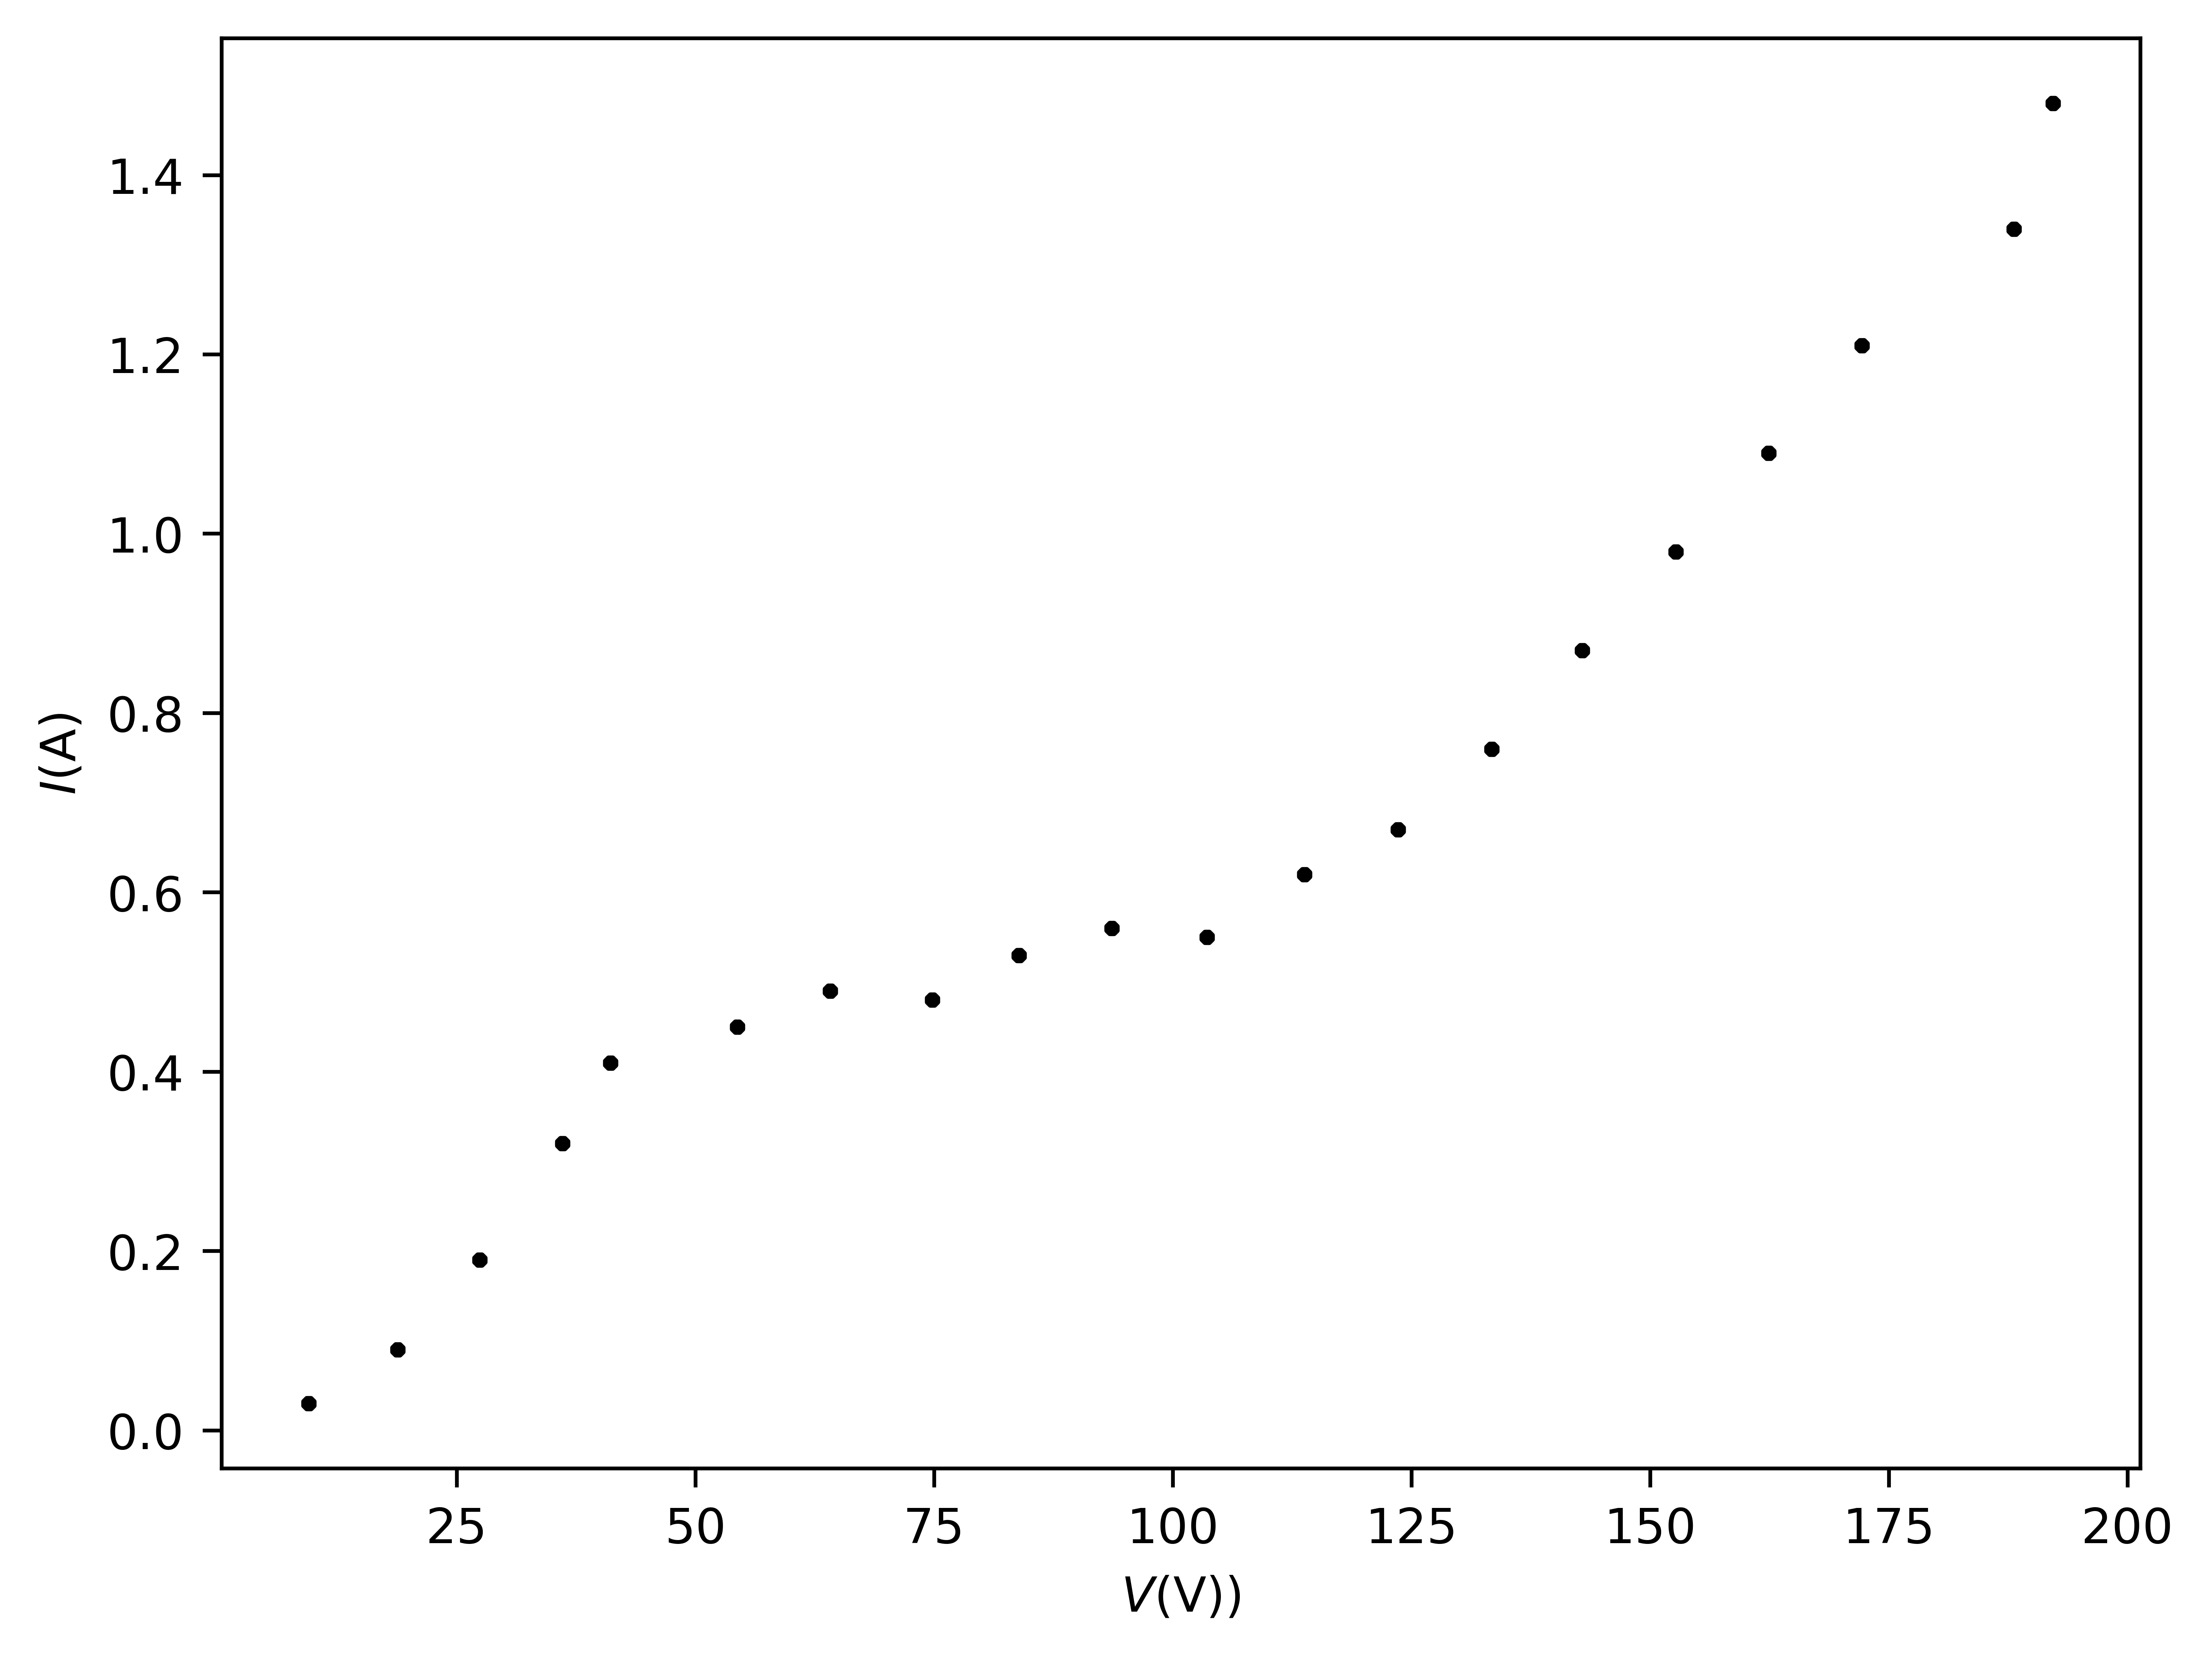
\includegraphics[width=0.45\textwidth]{figures/curva.png}
\end{center}

\section*{Conclusiones}
En las tablas 1 y 2 observamos que el montaje corto es más preciso para valores pequeños, como se ha predicho el el fundamento teórico. La comparción de los métodos para grandes resistecias no ha sido posible ya que en el montaje largo entre el voltímetro y resistencia bloqueaban toda la corriente.

En el circuito de las dos resistecias de $47\Omega$ se observa $V_1 + V_2 \approx V_34$ como era de esperar.

El valor de la resistencia obtenido con el multímetro difiere bastante de los de la Tabla 3, lo más seguro es que l multímetro utilice un voltaje muy bajo. Respecto a la curva característica de la bombilla, parece que la resistencia no es constante y depende del voltaje, esto se debe a que a medida que sube el voltaje el filamento de la bombilla se calienta y emite luz, es decir quita más energía a la corriente y por lo tanto genera más resistencia

\begin{thebibliography}{1}

  \bibitem{manual}Manual de la asignatura. Versión 3.7

  \bibitem{web}\url{https://uned-labo.netlify.app/practicas/te/5_practica_corriente_continua_2/prak5.html} 17/0672022

\end{thebibliography}
\end{multicols}
\end{document}